% !TEX encoding = UTF-8 Unicode
% REMEMBER TO SET LANGUAGE!
\documentclass[a4paper,10pt,norsk]{article}
\usepackage[utf8]{inputenc}
\usepackage[norsk]{babel}
% Standard stuff
\usepackage{amsmath,graphicx,varioref,verbatim,amsfonts,geometry}
% colors in text
\usepackage[usenames,dvipsnames,svgnames,table]{xcolor}
% Hyper refs
\usepackage[colorlinks]{hyperref}

% Document formatting
\setlength{\parindent}{0mm}
\setlength{\parskip}{1.5mm}

%Color scheme for listings
\usepackage{textcomp}
\definecolor{listinggray}{gray}{0.9}
\definecolor{lbcolor}{rgb}{0.9,0.9,0.9}

%Listings configuration
\usepackage{listings}
%Hvis du bruker noe annet enn python, endre det her for å få riktig highlighting.
\lstset{
	backgroundcolor=\color{lbcolor},
	tabsize=4,
	rulecolor=,
	language=python,
        basicstyle=\scriptsize,
        upquote=true,
        aboveskip={1.5\baselineskip},
        columns=fixed,
	numbers=left,
        showstringspaces=false,
        extendedchars=true,
        breaklines=true,
        prebreak = \raisebox{0ex}[0ex][0ex]{\ensuremath{\hookleftarrow}},
        frame=single,
        showtabs=false,
        showspaces=false,
        showstringspaces=false,
        identifierstyle=\ttfamily,
        keywordstyle=\color[rgb]{0,0,1},
        commentstyle=\color[rgb]{0.133,0.545,0.133},
        stringstyle=\color[rgb]{0.627,0.126,0.941}
        }
        
\newcounter{subproject}
\renewcommand{\thesubproject}{\alph{subproject}}
\newenvironment{subproj}{
\begin{description}
\item[\refstepcounter{subproject}(\thesubproject)]
}{\end{description}}

%Lettering instead of numbering in different layers
%\renewcommand{\labelenumi}{\alph{enumi}}
\renewcommand{\thesubsection}{\alph{subsection}}

%opening
\title{FYS-MEK 1110 - Oblig 1}
\author{Joakim Flatby}

\begin{document}

\maketitle
\section{}


%Oppg a
\subsection{)}

\begin{figure}[h!]
        \centering 
        \includegraphics[scale=1.0]{chart.png} 
        \caption{Free Body Diagram of a person running.(Drawn with draw.io)}
\end{figure}

%Oppg b
\subsection{)}
 
 Since acceleration is the double derivative og position, I can use Newtons second law to find an ecpression for acceleration, and then integrate it twice.
 
 \[F = ma\]
 \[a = \frac{F}{m}\]
 \[a = \frac{400N}{80kg} = 5m/s^{2}\]
 
 \[a(t) = v'(t)\]
 \[v(t) = \int a(t)  dt\]
 \[v(t) = \int 5dt\]
 \[v(t) = 5t\]
 
 \[x(t) = \int v(t) dt\]
\[x(t) = \int 5t dt\]
\[x(t) = 2.5t^{2}\] 
 
 %Oppg c
 \subsection{)}
 To find the time after 100 meters I just need to flip around my function for position and input 100 meters.
 \[x(t) = 2.5t^{2}\]
 \[t^{2} = \frac{x(t)}{2.5}\]
 \[t = \sqrt{\frac{x(t)}{2.5}}\]
 \[t = \sqrt{\frac{100}{2.5}}\]
 \[t = 6.32s\]
 
 %Oppg d
 \subsection{)}
 
 Expression for D and value of F given in the task:
 \[D = (1/2)pCdA(v-w)^{2}\]
 \[F = 400N\]
 
 Now I find the sum of horzontal forces by subracting D from F, and using Newtons second law(F=ma) I can find an expression for a
 
 \[\sum F_{x} = F - D\]
 \[= 400N - 0.5*1.293kg/m^{3}*1.2*0.45m^{2}v^{2} = m * a\]
 \[a(t) = \frac{400N - 0.5*1.293kg/m^{3}*1.2*0.45m^{2}v^{2}}{80kg}\]
 \[a(t) = \bigg( \frac{-0.6 * 1.293 * 0.45}{80}v(t)^{2} + 5 \bigg) m/s^{2}\]
 
 (I put 0 in for w in the air resistance formula since nothing else was specified)
 
 %Oppg e
 \subsection{)}
 
 \begin{figure}[h!]
        \centering 
        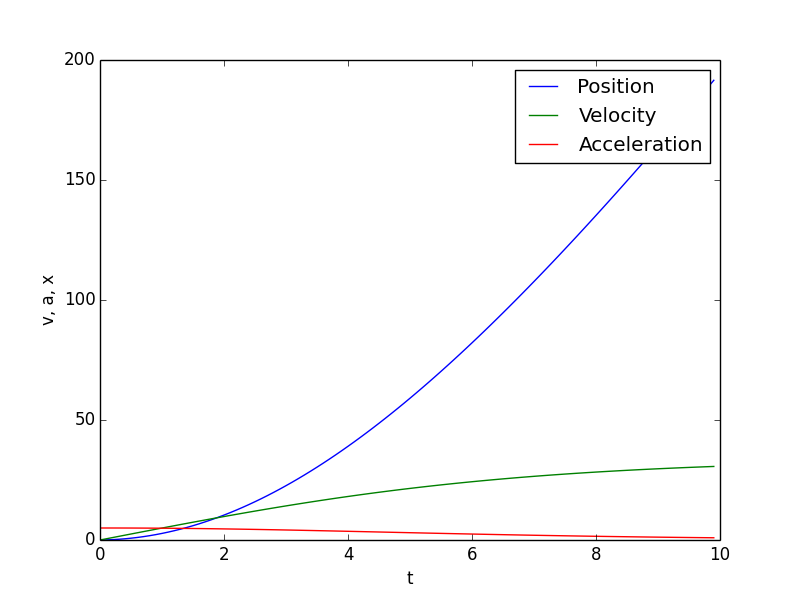
\includegraphics[scale=0.5]{taskE.png} 
        \caption{Graph plotting position, velocity and acceleration.}
\end{figure}
 
 \lstinputlisting{euler.py}
 
 %Oppg f
 \subsection{)}
 (See figure in task E) I added an if-statement to the for-loop that checks if x >= 100, and print the time when it is.
 It returns 6.8 seconds.
 
 %Oppg g
 \subsection{)}
  With the model given in this task terminal velocity is reached when the drag-force is equal to the driving force:
  \[F = D\]
  \[F = 1/2pCdAv^{2}_{T}\]
  \[2F = pCdAv^{2}_{T}\]
  \[\frac{2F}{pCdA} = v^{2}_{T}\]
  \[v_{T} = \sqrt{\frac{2F}{pCdA}}\]
 And this is what we were supposed to show.
 
 %Oppg h
 \subsection{)}
 
 %Oppg i
 \subsection{)}
 
 \begin{figure}[h!]
        \centering 
        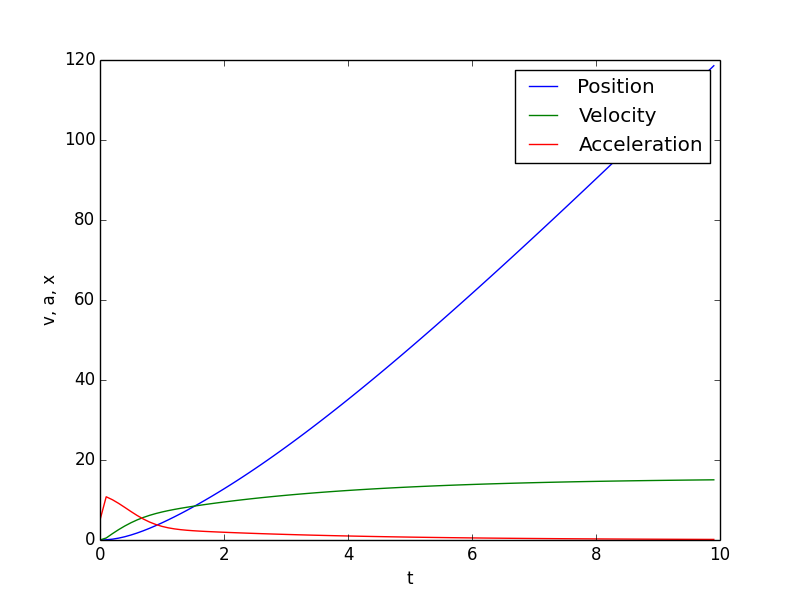
\includegraphics[scale=0.5]{taskI.png} 
        \caption{Graph plotting position, velocity and acceleration with a more realistic model.}
\end{figure}
 
 \lstinputlisting{euler2.py}

%Oppg j
\subsection{)}
After the changes he runs 100m in 8.7 seconds.
 
%Oppg k
\subsection{)}
The air resistance has a much less significant effect on the total force. It makes sense that a runners own physical limitations stop him before air resistance does.

\subsection{)}
The resulting time of the 100m run will remain approximately the same even with wind speeds of 1m/s or -1m/s. This correlates with the results of task K which said the air drag force is insignificant.

\end{document}
